% Propósito: comparar la suma de dos sinusoides de igual frecuencia y amplitud
% para tres diferencias de fase.
% Origen: y_1=cos(omega t), y_2=cos(omega t+Delta phi) y
% y_R=y_1+y_2, ecuaciones \eqref{eq:u3-superposicion} y
% \eqref{eq:u3-amplitud-resultante}.
% Curvas teóricas normalizadas; no representan datos medidos.
% Descripción accesible: tres paneles muestran dos señales y su suma. Con
% diferencia de fase cero, la suma duplica la amplitud; con pi sobre dos, la
% amplitud es raíz de dos; con pi, la suma es cero en todo instante.
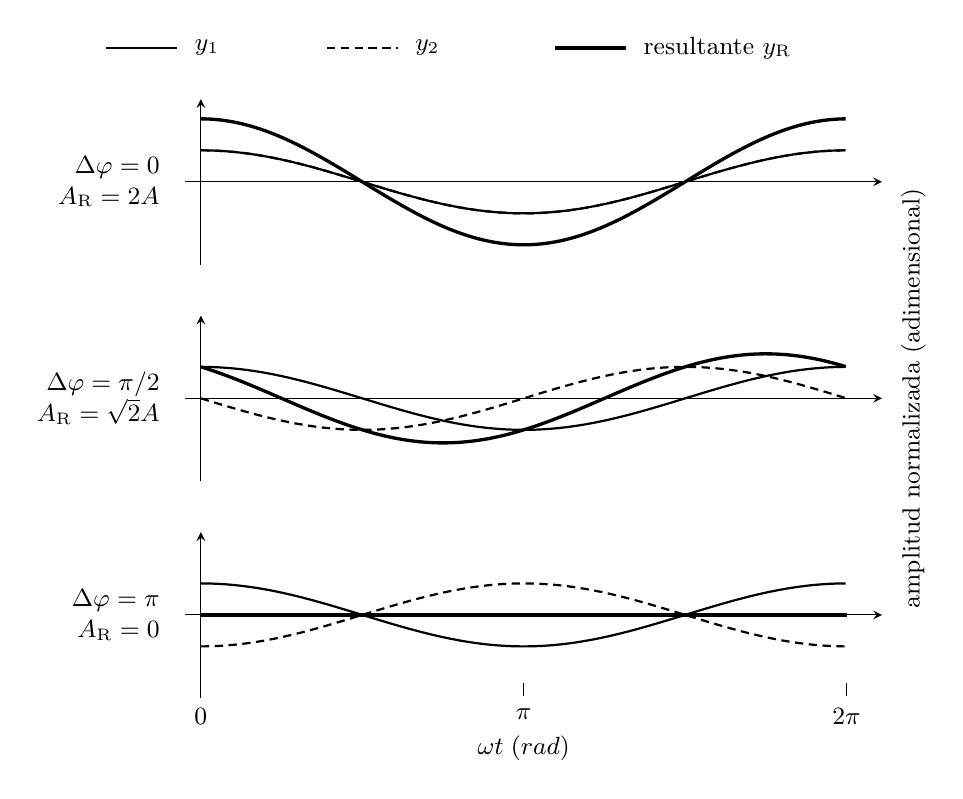
\begin{tikzpicture}[font=\small,>=stealth,x=1cm,y=1cm]
    % Leyenda.
    \draw[thick] (1.30,4.45) -- (2.20,4.45);
    \node[anchor=west] at (2.30,4.45) {\(y_1\)};
    \draw[thick,densely dashed] (4.10,4.45) -- (5.00,4.45);
    \node[anchor=west] at (5.10,4.45) {\(y_2\)};
    \draw[very thick] (7.00,4.45) -- (7.90,4.45);
    \node[anchor=west] at (8.00,4.45) {resultante \(y_\mathrm{R}\)};

    % Ejes comunes.
    \foreach \yy/\fase/\amp in {2.75/{0}/{2A},0/{\pi/2}/{\sqrt{2}A},-2.75/{\pi}/{0}}{
        \draw[->] (2.30,\yy) -- (11.15,\yy);
        \draw[->] (2.50,\yy-1.05) -- (2.50,\yy+1.05);
        \node[anchor=east,align=right] at (2.10,\yy)
            {\(\Delta\varphi=\fase\)\\\(A_\mathrm{R}=\amp\)};
    }

    % Caso Delta phi = 0.
    \draw[thick,samples=120,domain=0:1]
        plot ({2.50+8.20*\x},{2.75+0.40*cos(360*\x)});
    \draw[thick,densely dashed,samples=120,domain=0:1]
        plot ({2.50+8.20*\x},{2.75+0.40*cos(360*\x)});
    \draw[very thick,samples=120,domain=0:1]
        plot ({2.50+8.20*\x},{2.75+0.80*cos(360*\x)});

    % Caso Delta phi = pi/2.
    \draw[thick,samples=120,domain=0:1]
        plot ({2.50+8.20*\x},{0.40*cos(360*\x)});
    \draw[thick,densely dashed,samples=120,domain=0:1]
        plot ({2.50+8.20*\x},{0.40*cos(360*\x+90)});
    \draw[very thick,samples=120,domain=0:1]
        plot ({2.50+8.20*\x},{0.40*(cos(360*\x)+cos(360*\x+90))});

    % Caso Delta phi = pi.
    \draw[thick,samples=120,domain=0:1]
        plot ({2.50+8.20*\x},{-2.75+0.40*cos(360*\x)});
    \draw[thick,densely dashed,samples=120,domain=0:1]
        plot ({2.50+8.20*\x},{-2.75+0.40*cos(360*\x+180)});
    \draw[very thick] (2.50,-2.75) -- (10.70,-2.75);

    % Etiquetas del eje de fase.
    \foreach \q/\lab in {0/{0},0.5/{\pi},1/{2\pi}}{
        \pgfmathsetmacro{\xx}{2.50+8.20*\q}
        \draw (\xx,-3.78) -- (\xx,-3.62);
        \node[below] at (\xx,-3.82) {\(\lab\)};
    }
    \node at (6.60,-4.45) {\(\omega t\;(\text{rad})\)};
    \node[rotate=90] at (11.55,0)
        {amplitud normalizada (adimensional)};
\end{tikzpicture}
